%************************************************
\chapter[Species Abundance Distributions and trophic structure]{On the variability of Species Abundance Distributions with trophic guild and community structure}\label{ch:SAD}
%************************************************

%\tikz[remember picture,overlay] \node[opacity=0.3,inner sep=0pt] at (current page.center){\includegraphics[width=\paperwidth,height=\paperheight]{./Figures/cover/barco_oceano.png}};
\tikz[remember picture,overlay] \node[opacity=0.3,inner sep=0pt] at ([yshift=3cm,xshift=2cm]current page.center){\includegraphics[width=\paperwidth,height=\paperheight]{./Figures/cover/barco_oceano.png}};
\clearpage

\section*{Abstract}

Species Abundance Distributions (SADs) are one of the strongest generalizations in community ecology, but their variation across trophic levels remains largely unexplored. I study the variation in SAD metrics across trophic guilds, using a theoretical model and a compilation of empirical datasets. First, I develop a model that allows tracking the variations in abundances across trophic guilds, controlling for species richness and network connectance. The theoretical results show that evenness is highest for herbivores, and decreases in omnivore and carnivore guilds. The richness and connectance of the community network are also negatively correlated with guild evenness. Second, I compare the empirical SADs of 226 terrestrial plant communities and 497 mammal communities comprising species grouped in three general trophic guilds (herbivores, omnivores, and carnivores). Sampled plant communities are significantly less even and more skewed than mammal ones. There are no significant differences in SAD metrics between the different mammal guilds, but carnivores are comparatively rare (i.e. have a higher proportion of species than individuals), whereas omnivores are comparatively more common. Species richness has a positive effect on both evenness and skewness, and spatial and temporal extent have negative effects on evenness and do not affect skewness. I argue that the difference between plant and mammal guilds can be related to higher niche availability in animals than in plants, that decreases the importance of competitive exclusion in mammal guilds. As no systematic differences were found between the SADs of mammal herbivores, omnivores, and carnivores, this may indicate similar niche availability, when averaged across habitat types, for the different animal trophic guilds.

\section{Introduction}

Most species, in any ecological community, are comparatively rare, and only a few of them are very abundant. This empirical observation is one of the few true universal laws in ecology, a pattern that is observed in all kinds of communities and guilds, from small arthropods \citep{Basset1991} to tropical trees \citep{He1997}. The Species Abundance Distribution (SAD) describes precisely this variation in species abundances within a given assemblage.

The information contained in SADs, aside from its theoretical interest in understanding community dynamics \citep{Hillebrand2008}, can be of interest for conservation and management \citep{Matthews2015} or for estimating ecosystem functions such as primary productivity \citep{Wilsey2000}. It is therefore important to understand which are the main axes of variability in SAD shape across guilds, and what are the ecological processes underlying this variability. So far, important efforts have been devoted to understand variation in species abundances across enviromental gradients \citep{Ulrich2016, Passy2016}, levels of disturbance \citep{Komonen2017}, spatiotemporal scales \citep{Borda-de-Agua2012}, or multiple factors combined \citep{Arellano2017}. Intrinsic differences in species-level traits among the species that make up the community will also be reflected in the SAD. For example, core and satellite species of an ecosystem are likely to differ in their intrinsic abundances regardless of other factors \citep{Magurran2003}, and the degree of trophic or habitat specialization of different species may also be related to their relative abundances \citep{Labra2005, Matthews2015}.

Despite these significant advances, in the debates on the mechanisms that shape SADs, virtually all theories and hypothesis that relate SAD shape to ecological processes at the local scale refer to horizontal communities, i.e. communities of a single trophic level. Thus, these theories emphasize the role of either neutral dispersal and drift \citep{Hubbell2001} or horizontal selection \citep{Vellend2016}. But natural communities form a complex network of species linked by different types of biotic interactions both horizontally (within a given trophic guild) and vertically (across trophic guilds, Fig. \ref{fig:fig4.1}). The influence of the interaction topology on the abundance patterns of the different guilds of a community has, to my knowledge, never been explored systematically.

\begin{figure}[ht!]
\centering
\includegraphics[width=0.5\textwidth,height=\textheight,keepaspectratio]{./Figures/chapter04/Fig_1.png}
\caption[Schematic multi-trophic community]{\color{Gray}A schematic ecological community with three disjoint trophic guilds. The areas within the ellipses represent the domain of horizontal community ecology that is the subject of most SAD studies, focusing on intra-guild interactions (dashed grey lines) and assuming that interactions with other guilds (full grey lines) are negligible. In this study, I focus on how interactions across guilds drive variations in SAD metrics.}\label{fig:fig4.1}
\end{figure}

In complex, multitrophic ecological communities, trophic guilds (sensu \citealt{Fauth1996}) differ in fundamental properties that can potentially be reflected in their associated abundace distributions. First, several studies have demonstrated that basic descriptors, such as biomass or species richness, vary predictably with trophic level (e.g. \citealt{Lindeman1942,Odum1957,Turney2016}). Focusing on the relationship between two adjacent trophic levels, \cite{Hatton2015} showed that the biomass of empirical guilds of herbivores and their associated predators scales generally with a power-law of exponent 3/4. They also showed that, in their data, the relationship between mean body mass and community biomass is non-significant for most of the functional groups they studied. As such, if body mass varies in a similar fashion in different trophic levels, the scaling in biomass should also be reflected in a scaling on number of individuals at each trophic level, as foretold by Ramón \cite{Margalef1980}.

Other patterns associated to the distribution of abundances, such as species rarity or the degree of dominance, can potentially vary across different trophic guilds, but empirical evidence is scarce. In a study of macroinvertebrate communities, predators showed a higher proportion of species than of individuals in the overall community \citep{Spencer2000}, pointing to a higher rarity in predator species. Furthermore, \cite{Spencer2000} showed that predator and non-predator species did not vary significantly in the ratios of dominance of the most abundant species. More recently, \cite{Dornelas2011} showed that relative dominance decreased consistently with increasing richness in communities of freshwater fish.

Overall, these lines of evidence suggest a complex, combined influence of the richness and trophic position of a guild on its abundance patterns. In a first approximation, the number of different resources available to a given trophic guild and the partition of these resources among its constituent species \citep{Tokeshi1990, Sugihara2003} will ultimately drive the guild's SAD. As the trophic interactions among guilds are encoded in the topological structure of the community food web, this structure is likely to play a role in modulating SAD variability across guilds.

Analyzing abundance distributions in communities comprising several trophic guilds is complicated further by a number of factors. For example, movement capacity generally increases with trophic position \citep{McCann2005}, and in turn, it significantly influences SADs and their variation with sampled area \citep{Borda-de-Agua2017}. Therefore, different trophic guilds in the same community will likely require varying sampling areas in order to obtain their abundance patterns in a consistent fashion (see also \citealt{Holt1999}). Another issue that needs to be considered when comparing trophic guilds of different communities is precisely how to divide species among guilds in a general way. Broad categories such as herbivores/omnivores/carnivores provide groupings applicable to communities of different ecosystem types, but are likely to be too general, lumping together species with very different ecologies. On the other hand, clearly defined guilds for a given community type (e.g. sap-feeding insects in salt marsh grasses) will be too specific to allow comparisons with guilds from other ecosystem types. Therefore, a robust analysis of the role of trophic guild in SAD metrics needs to control for (1) the variations in richness across guilds, (2) the spatial and temporal extent of the data collection, and (3) the process of defining trophic guilds in a general and informative way.

Here I approach the general question of whether SAD metrics vary predictably across trophic guilds, in two complementary ways. First, I combine a model of food web structure with niche apportionment schemes for studying how SADs of different trophic guilds vary in model communities with varying network structures. Second, I analyze SAD patterns of two well-resolved datasets on community abundances of plants \citep{Phillips2002} and mammals \citep{Thibault2011}. I compare SAD patterns of plant communities and three mammal trophic guilds, controlling for guild richness, spatial and temporal extent of the data collection.

\section{Methods}

\subsection*{The relationship between SAD properties and trophic guild: A theoretical model}

Analyses of species abundance distributions are based, on their first stage, on the grouping of species that are supposed to share certain properties of interest, such as taxonomic relatedness, spatial location or resource use \citep{Fauth1996}. As a starting point, I focus on the role of the different trophic guilds in a local multi-trophic community. Intuitively, the variability in number of individuals between species of a given trophic guild will depend on inter-specific variation in both species-level traits and resource use. Assuming, as a working hypothesis, that the main difference between species within a guild is in their competitive ability to acquire resources, it can be hypothesized that the degree of resource overlap between the species will play an important role in determining their variations in abundance \citep{Sugihara2003}. Consider a single herbivore species that is preyed upon by a number of predators. All else being equal, the partition of the prey resource will be driven by the competitive ability of these predators, and will be reflected in their own abundances (an energetic view of abundance, \citealt{Isaac2013}). When an arbitrary number of prey species can be exploited by the predators, the specialization level of the predators will influence the degree of exploitative competition between them, and indirectly its distribution of abundances. In network terminology, the level of specialization of a species is given by its degree, the number of interactions in which it engages, and indirectly, by the connectance of the network, the ratio of realized to potential interactions in it.

This qualitative hypothesis can be more precisely formulated by combining models of network structure and resource partitioning schemes. In particular, I generated food webs with varying connectance and richness values. Then, I grouped their constituent species in trophic guilds, calculated the expected abundances of each species according to a resource apportionment model, and compared the resulting distribution of abundances of the different guilds. There is a long tradition of resource partitioning models along a single axis, and here I implemented the Random Fraction model, which has been shown to fit empirical datasets reasonably well \citep{Tokeshi1990}.

In this scheme, the resource is divided sequentially into fractions, until each consumer is given a fraction of the available resource. At each step, the fraction that is divided is randomly chosen, so that either the biggest fraction could be divided, leading to more equitable distributions, or the smallest fraction, leading to a bigger share for a single species. This scheme generates dominance hierarchies intermediate between a purely \textit{dominance preemption} scheme, in which dominant species always gets the higher share of the resource, and a \textit{dominance decay} scheme, in which resources are distributed most equitably \citep{Tokeshi1990}. Food webs were generated using a modified version of the niche model \citep{Williams2000}. The original niche model takes a single niche axis in which all species are placed to generate trophic links allowing for a certain degree of intraguild predation (the original formulation is given in \citealt{Williams2000}, and its particularities with respect to other food web models are explored, for example, in \citealt{Dunne2006}). The network topologies generated with it are similar in terms of goodness-of-fit to those from more complex models \citep{Williams2008}, so it remains an appropriate model for generating food web structures in the absence of detailed information on trait structure \citep{Gravel2016}. One of its limitations, however, is the systematic underestimation of the proportion of primary producers and herbivores compared to empirical food webs. In this study, I imposed a minimum fraction of 0.2 of primary producers in the generated food webs. Furthermore, I removed all directed cycles from the web, in order to make the propagation of biomass across species feasible. For each cycle (i.e. a series of nodes and links that eventually form a closed chain), I selected one of its constituent links randomly and assigned the resource to be a basal species. These two modifications to the original model are likely to modify some emergent properties of the network structure, but the resulting connectance of the generated food webs is maintained, and the proportion of primary producers and herbivores is increased with respect to the original formulation. I grouped the species in primary producers, herbivores (i.e. species whose only feeding sources are primary producers), omnivores (species that feed in both primary producers and other species), and carnivores (species that do not feed on primary producers). In order to obtain the abundances of the species in the food web, the abundances of the basal species need to be specified beforehand, as this model represents a static bottom-up approach. I generated basal abundances from a Weibull distribution with scale = 4.7 and shape = (0.15,0.2), derived as the average best fit from the 226 sites of the GENTRY dataset (see \textit{datasets} section).

I considered three levels of species richness (50, 100, and 200 species), and three levels of network connectance (0.1, 0.2, and 0.3). For each combination of richness and connectance, I generated 1000 networks and quantified the evenness and skewness of the SAD of the different trophic guilds (see next section).

I analyzed the variability of SAD metrics with connectance, species richness and trophic guild by using regression models. In particular, I used linear mixed-effect models (R package ``lme4'', \citealt{Bates2015}) with richness, connectance, and trophic guild as fixed effects, and replicate (e.g. the 1000 simulated networks for each combination of richness and connectance) as a random effect. As I am not interested in predictions from this model, but rather in the effect of the different predictors, I did not perform model selection procedures.

\subsection*{Metrics for quantifying Species Abundance Distributions}

Methodologically, the comparison of SADs is still an unresolved problem in community ecology: there is no standard method for comparing SAD shape of guilds with arbitrary numbers of species or individuals, with most comparisons being qualitative \citep{McGill2007} or being made between relatively similar communities that don’t differ much in richness or size (e.g. samples from polluted and unpolluted habitats, \citealt{Matthews2015}). In order to assess the variability between SADs in a general way, robust metrics need to be developed that are independent of number of species and individuals, i.e. that reflect solely the variability in the shape of the distribution. In this study, I assess the variability in SAD shape through two complementary metrics, that quantify the evenness and the skewness of the distribution.

Evenness is defined after the ``Hill number'' of species diversity, also known as the effective number of species \citep{Jost2006}. This diversity metric represents how many equally-abundant species would give the observed mean proportional species abundance \citep{Tuomisto2012}. The evenness metric derived from the effective number of species has a series of desirable properties, summarized in \cite{Smith1996}. It is also conceptually similar to the variance of a distribution, but the evenness metric has the advantage of having a clear ecological meaning. The skewness metric is simply a robust version of the third moment of a statistical distribution \citep{Brys2004}. Throughout this study, I apply these metrics to the natural abundances of both the simulated and compiled data.

\subsection*{Empirical SAD patterns across trophic guilds}

\subsubsection*{Datasets}

I analysed two datasets that report species abundances at different sites along with the spatial and temporal smapling effort from each site. Gentry's Forest Transect Dataset (GENTRY, \citealt{Phillips2002}) compiles observations from 226 sites of 0.1 ha in temperate and tropical forests across the globe. At each site, Gentry and collaborators collected the abundance of all plant species with stem diameters at breast height equal to or exceeding 2.5 cm. The second dataset is the Mammal Community Database (MCDB, \citealt{Thibault2011}), which provides abundances of 660 mammal species in 940 sites, alongside detailed information about the sampling and context of the local community. Rank-abundance curves of one GENTRY site and four MCDB sites are shown in Fig. \ref{fig:fig4.2}.

Another global dataset on mammal foraging habits \citep{Wilman2014} was used to derive trophic guild categorizations for every species in the MCDB dataset. I assigned each species to one among three general trophic guilds: (1) herbivores (including folivores, granivores, frugivores, and nectarivores); (2) omnivores, and (3) carnivores (feeding on invertebrates, vertebrates, fish, and carrion). Herbivores and carnivores are species that have at least a 70\% of their diet from plant or animal origin, respectively, and species whose diet is $< 70\%$ herbivore or carnivore are labelled omnivores. While more detailed trophic guild distinctions are possible, the representativeness of the different categories varies drastically (e.g. there are only 22 mainly frugi/nectarivore species versus 324 foli/granivore ones). In a basic categorization such as the one presented here, the three trophic guilds are well represented (374 herbivores, 145 omnivores, 179 carnivores).

\begin{figure}[ht!]
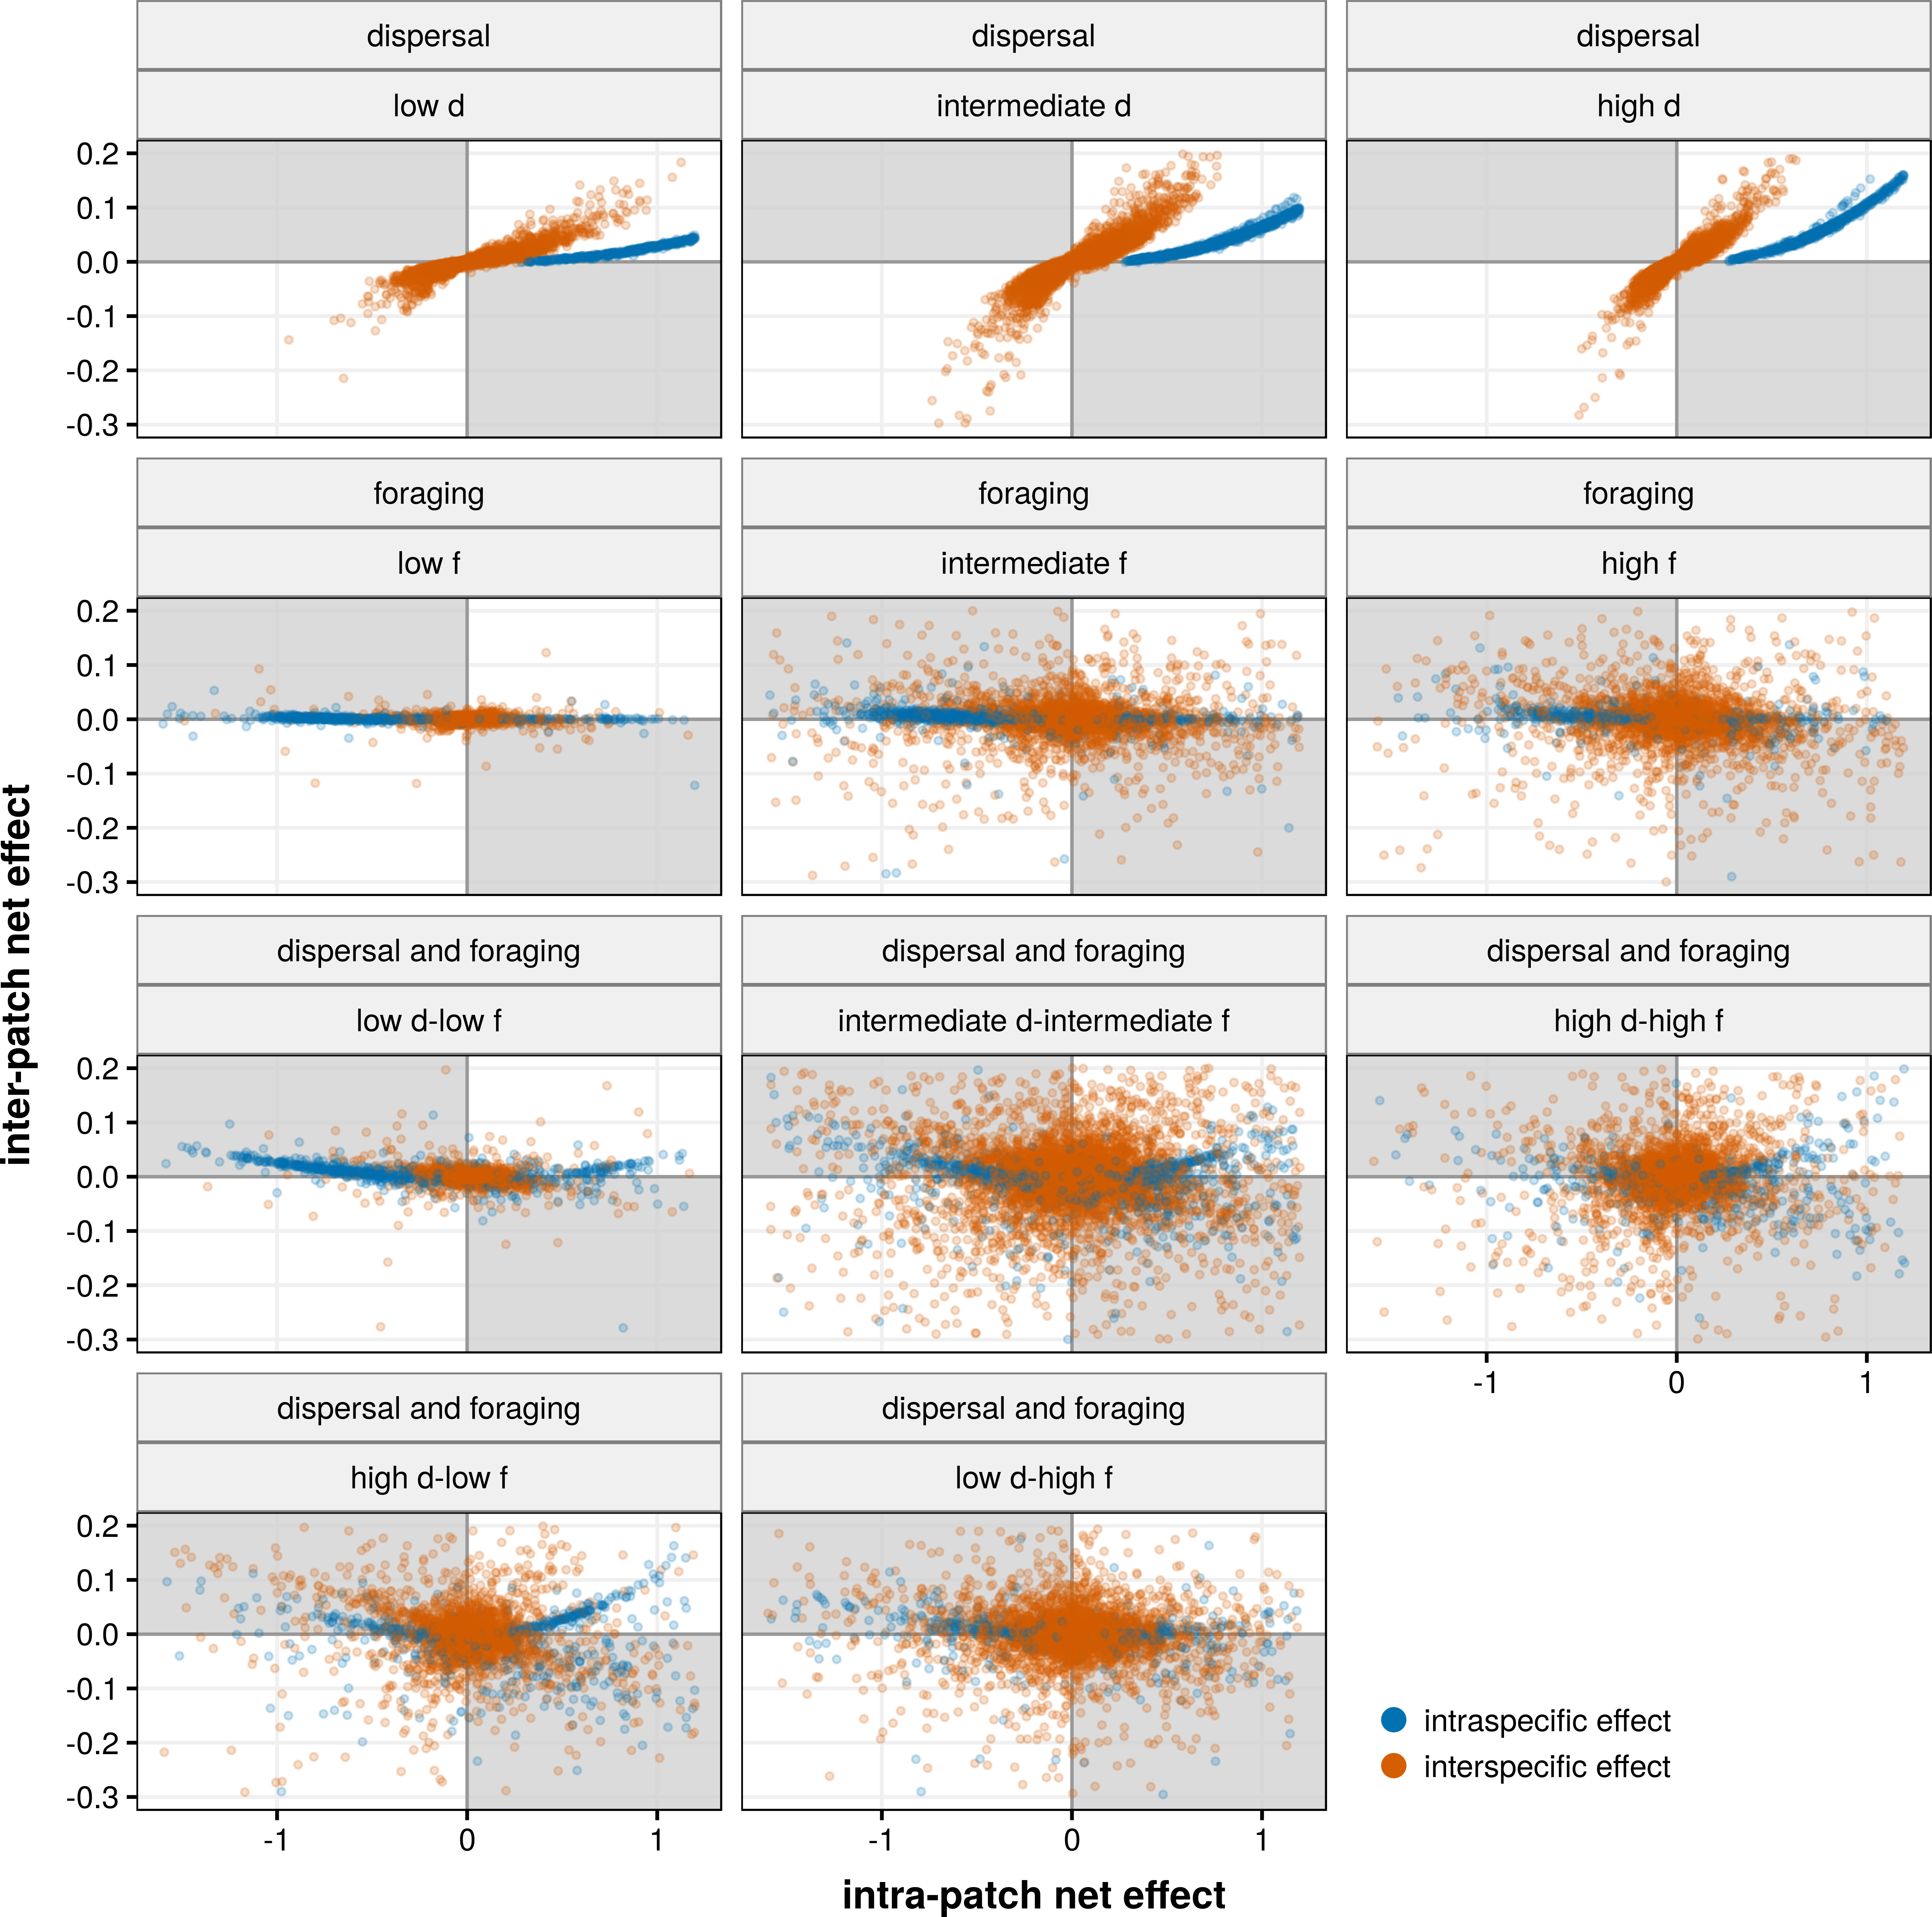
\includegraphics[width=\textwidth,height=\textheight,keepaspectratio]{./Figures/chapter04/Fig_2.png}
\caption[Five empirical rank-abundance curves]{\color{Gray}Rank-abundance curves for five sites of the empirical datasets. The leftmost panel shows a curve from a GENTRY site, the other four are sampling sites of the MCDB dataset. }\label{fig:fig4.2}
\end{figure}

\subsubsection*{Statistical analyses}

I calculated the evenness and skewness metrics of each guild at sites in which there are at least three species of that guild, in order to avoid potential biases (for example, a guild of a single species is completely even, or a guild of two species is never skewed). The variation of the SAD metrics with trophic guild was analyzed via statistical models. Evenness values are bounded within the interval [0,1], so a beta regression is an appropriate choice for modelling such bounded data, given the flexibility of the beta distribution. I transformed the evenness values in order to obtain data without proper zeroes and ones, i.e. bounded in (0,1), following \cite{Smithson2006}, and applied a beta regression with trophic guild, species richness, temporal extent and spatial extent as predictors. In particular, I used the R implementation of the GAMLSS family of models \citep{Rigby2005}, which allows probability density functions to be specified by any number of parameters, themselves functions of the independent variables. I modelled the evenness probability density function with two parameters $\mu$ and $\sigma$, named the \textit{location} and \textit{scale} parameters. These parameters are related to the parameterization of the beta distribution in terms of two shape parameters $\alpha$ and $\beta$ in the following way:

\begin{align}%\label{eq:eq4.3}
& \mu = \frac{\alpha}{\alpha + \beta} \\
& \sigma = \frac{1}{\alpha + \beta + 1}
\end{align}

Then, given a random variable $Y \sim D(\mu,\sigma)$, the mean and variance of the beta distribution in these terms is:

\begin{align}\label{eq:eq4.4}
& E(y) = \mu \\
& Var(y) = \sigma^2 * \mu * (1-\mu)
\end{align}

For the final model, I selected the link functions of $\mu$ and $\sigma$, and the final set of predictors, via AIC model selection.

Skewness presented a clearly bimodal distribution, with peaks at 0 and 1. Due to the difficulty of modelling such continuous bimodal data, I opted for categorizing the response into three levels of skewness: highly negative, low skewness, and highly positive, represented by the intervals [-1,-0.5), [-0.5,0.5], and (0.5,1]. This response was modelled via a multinomial regression with the same set of predictors as the evenness metric, and AIC model selection was also performed to obtain the final set of predictors.

For the MCDB dataset, it is common to observe species from two or more trophic guilds at the same site (Fig. \ref{fig:fig4.2}). It is therefore possible to calculate the rarity of each guild as the difference between its proportion of individuals and its proportion of species in the local communities \citep{Spencer2000}. Furthermore, to complement this calculation, I obtained the relative dominance value of each guild at each site, measured as the abundance of the most abundant species divided by the summed abundances of its guild \citep{Spencer2000, Dornelas2011}.

\section{Results}

\subsection*{Theoretical model}

Evenness and skewness metrics show contrasting responses to variations in trophic guild, richness and connectance (Tables \ref{tab:tab4.1} and \ref{tab:tab4.2}, see Fig. \ref{fig:fig4.3} for a subset of the results). After a high increase in evenness from primary producers to herbivores, the metric decreases on average with trophic guild. Likewise, richness displays a negative relationship with evennes, whereas connectance shows a more complex relationship, with minimum overall evenness observed at intermediate levels of connectance (Table \ref{tab:tab4.1}). Skewness, in turn, displays almost opposite trends: it increases with increasing trophic position, richness, and connectance (Table \ref{tab:tab4.2}).

\begin{figure}[htbp!]
\includegraphics[width=\textwidth,height=\textheight,keepaspectratio]{./Figures/chapter04/Fig_3.png}
\caption[Model evenness and skewness]{\color{Gray}Evenness and skewness values for the trophic guilds of simulated networks. In this figure, each dot represents one realization of a network with richness = 100 and connectance = 0.2. Note that the abundances predicted by the model correspond to the three consumer levels, whereas abundances of primary producers are inputs to the model, and are shown for reference. Black circles represent the centroid of the two-dimensional distributions.}\label{fig:fig4.3}
\end{figure}

\clearpage
\begin{landscape}
\begin{table}[ht!]
\centering
\caption[Coefficients from evenness regression in simulated networks]{\color{Gray}Estimated regression parameters, standard errors, t-statistic values and p-values for the mixed effect model \textit{evenness $\sim$ richness + connectance + trophic guild + random(replicate)} of the theoretical model. $\sigma_{replicate}$ is $5.3*10^{-8}$, and the $r^2$ of the model is 0.4}\label{tab:tab4.1}
\begin{tabular}{llllll}
\hline
Variable & Estimate & Std. Error &         df & t value & p-value \\
\hline
(Intercept)            &  0.41 & $1.848*10^{-3}$ & $2.63*10^{4}$ & 221.871 & $<0.05$ \\
richness-100      & -0.091 & $1.72*10^{-3}$ &  $2.63*10^{4}$ & -53.237 & $<0.05$ \\
richness-200      & -0.155 & $1.72*10^{-3}$ &  $2.63*10^{4}$ & -89.997 & $<0.05$ \\
connectance-0.2   & -0.007 & $1.7*10^{-3}$ &  $2.63*10^{4}$ & -4.351 & $<0.05$ \\
connectance-0.3   &  0.007 & $1.73*10^{-3}$ &  $2.63*10^{4}$ & 3.773 & $<0.05$ \\
trophic.guild-omnivores & -0.079 & $1.7*10^{-3}$ & $2.63*10^{4}$ & -46.453 & $<0.05$ \\
trophic.guild-carnivores & -0.167 & $1.73*10^{-3}$ & $2.63*10^{4}$ & -96.437 & $<0.05$ \\
\hline
\end{tabular}

\end{table}

\begin{table}[ht!]
\centering
\caption[Coefficients from skewness regression in simulated networks]{\color{Gray}Estimated regression parameters, standard errors, t-statistic values and p-values for the mixed-effects model \textit{skewness $\sim$  richness + connectance + trophic guild + random(replicate)} of the theoretical model. $\sigma_{replicate}$ is 0.0032, and the $r^2$ of the model is 0.24}\label{tab:tab4.2}
\begin{tabular}{llllll}
\hline
Variable & Estimate & Std. Error &         df & t value & p-value \\
\hline
(Intercept)       & 0.561 &  $3.65*10^{-3}$ & $1.9*10^{4}$ & 153.603 & $<0.05$ \\
richness-100      & 0.117 &  $3.39*10^{-3}$ & $2.5*10^{4}$ & 34.574 & $<0.05$ \\
richness-200      & 0.177 &  $3.4*10^{-3}$ & $2.5*10^{4}$ &  51.957 & $<0.05$ \\
connectance-0.2   & 0.019 &  $3.36*10^{-3}$ & $2.53*10^{4}$ &   5.674 & $<0.05$ \\
connectance-0.3   & 0.0048 &  $3.42*10^{-3}$ & $2.53*10^{4}$ &   1.414  &  0.157  \\
trophic.guild-omnivores & 0.086 &  $3.36*10^{-3}$ & $2.53*10^{4}$ &  25.739  & $<0.05$ \\
trophic.guild-carnivores & 0.253 &  $3.43*10^{-3}$ & $2.54*10^{4}$ &  73.909  & $<0.05$ \\
\hline
\end{tabular}

\end{table}

\end{landscape}

\FloatBarrier

\subsection*{Empirical datasets}

The statistical model for evenness included all the original predictors (trophic guild, richness, spatial extent and temporal extent, Table \ref{tab:tab4.3}). Plant guilds were the less even ones overall, showing significant differences with all other guilds (panel (a) of Fig. \ref{fig:fig4.4}, Appendix A.4.1: Table A.4.1.1). Among mammal guilds, herbivores show the highest average evenness, after which it further decreases with increasing trophic rank, although the differences are non-significant (Appendix A.4.1: Table A.4.1.1). This overall pattern of a significant increase from primary producers to consumers followed by a sustained decrease is qualitatively similar to the patterns obtained with the theoretical model, although the evenness values of the theoretical model are much lower than those of the empirical datasets (compare Figs. \ref{fig:fig4.3} and \ref{fig:fig4.4}). Richness has a positive effect on evenness, while also decreasing its variability (compare the sign of $\mu$ and $\sigma$ richness parameters), whereas increasing temporal and spatial extent has a negative effect on mean evenness, and no effect on its variability (Table \ref{tab:tab4.3}).

\begin{figure}[ht!]
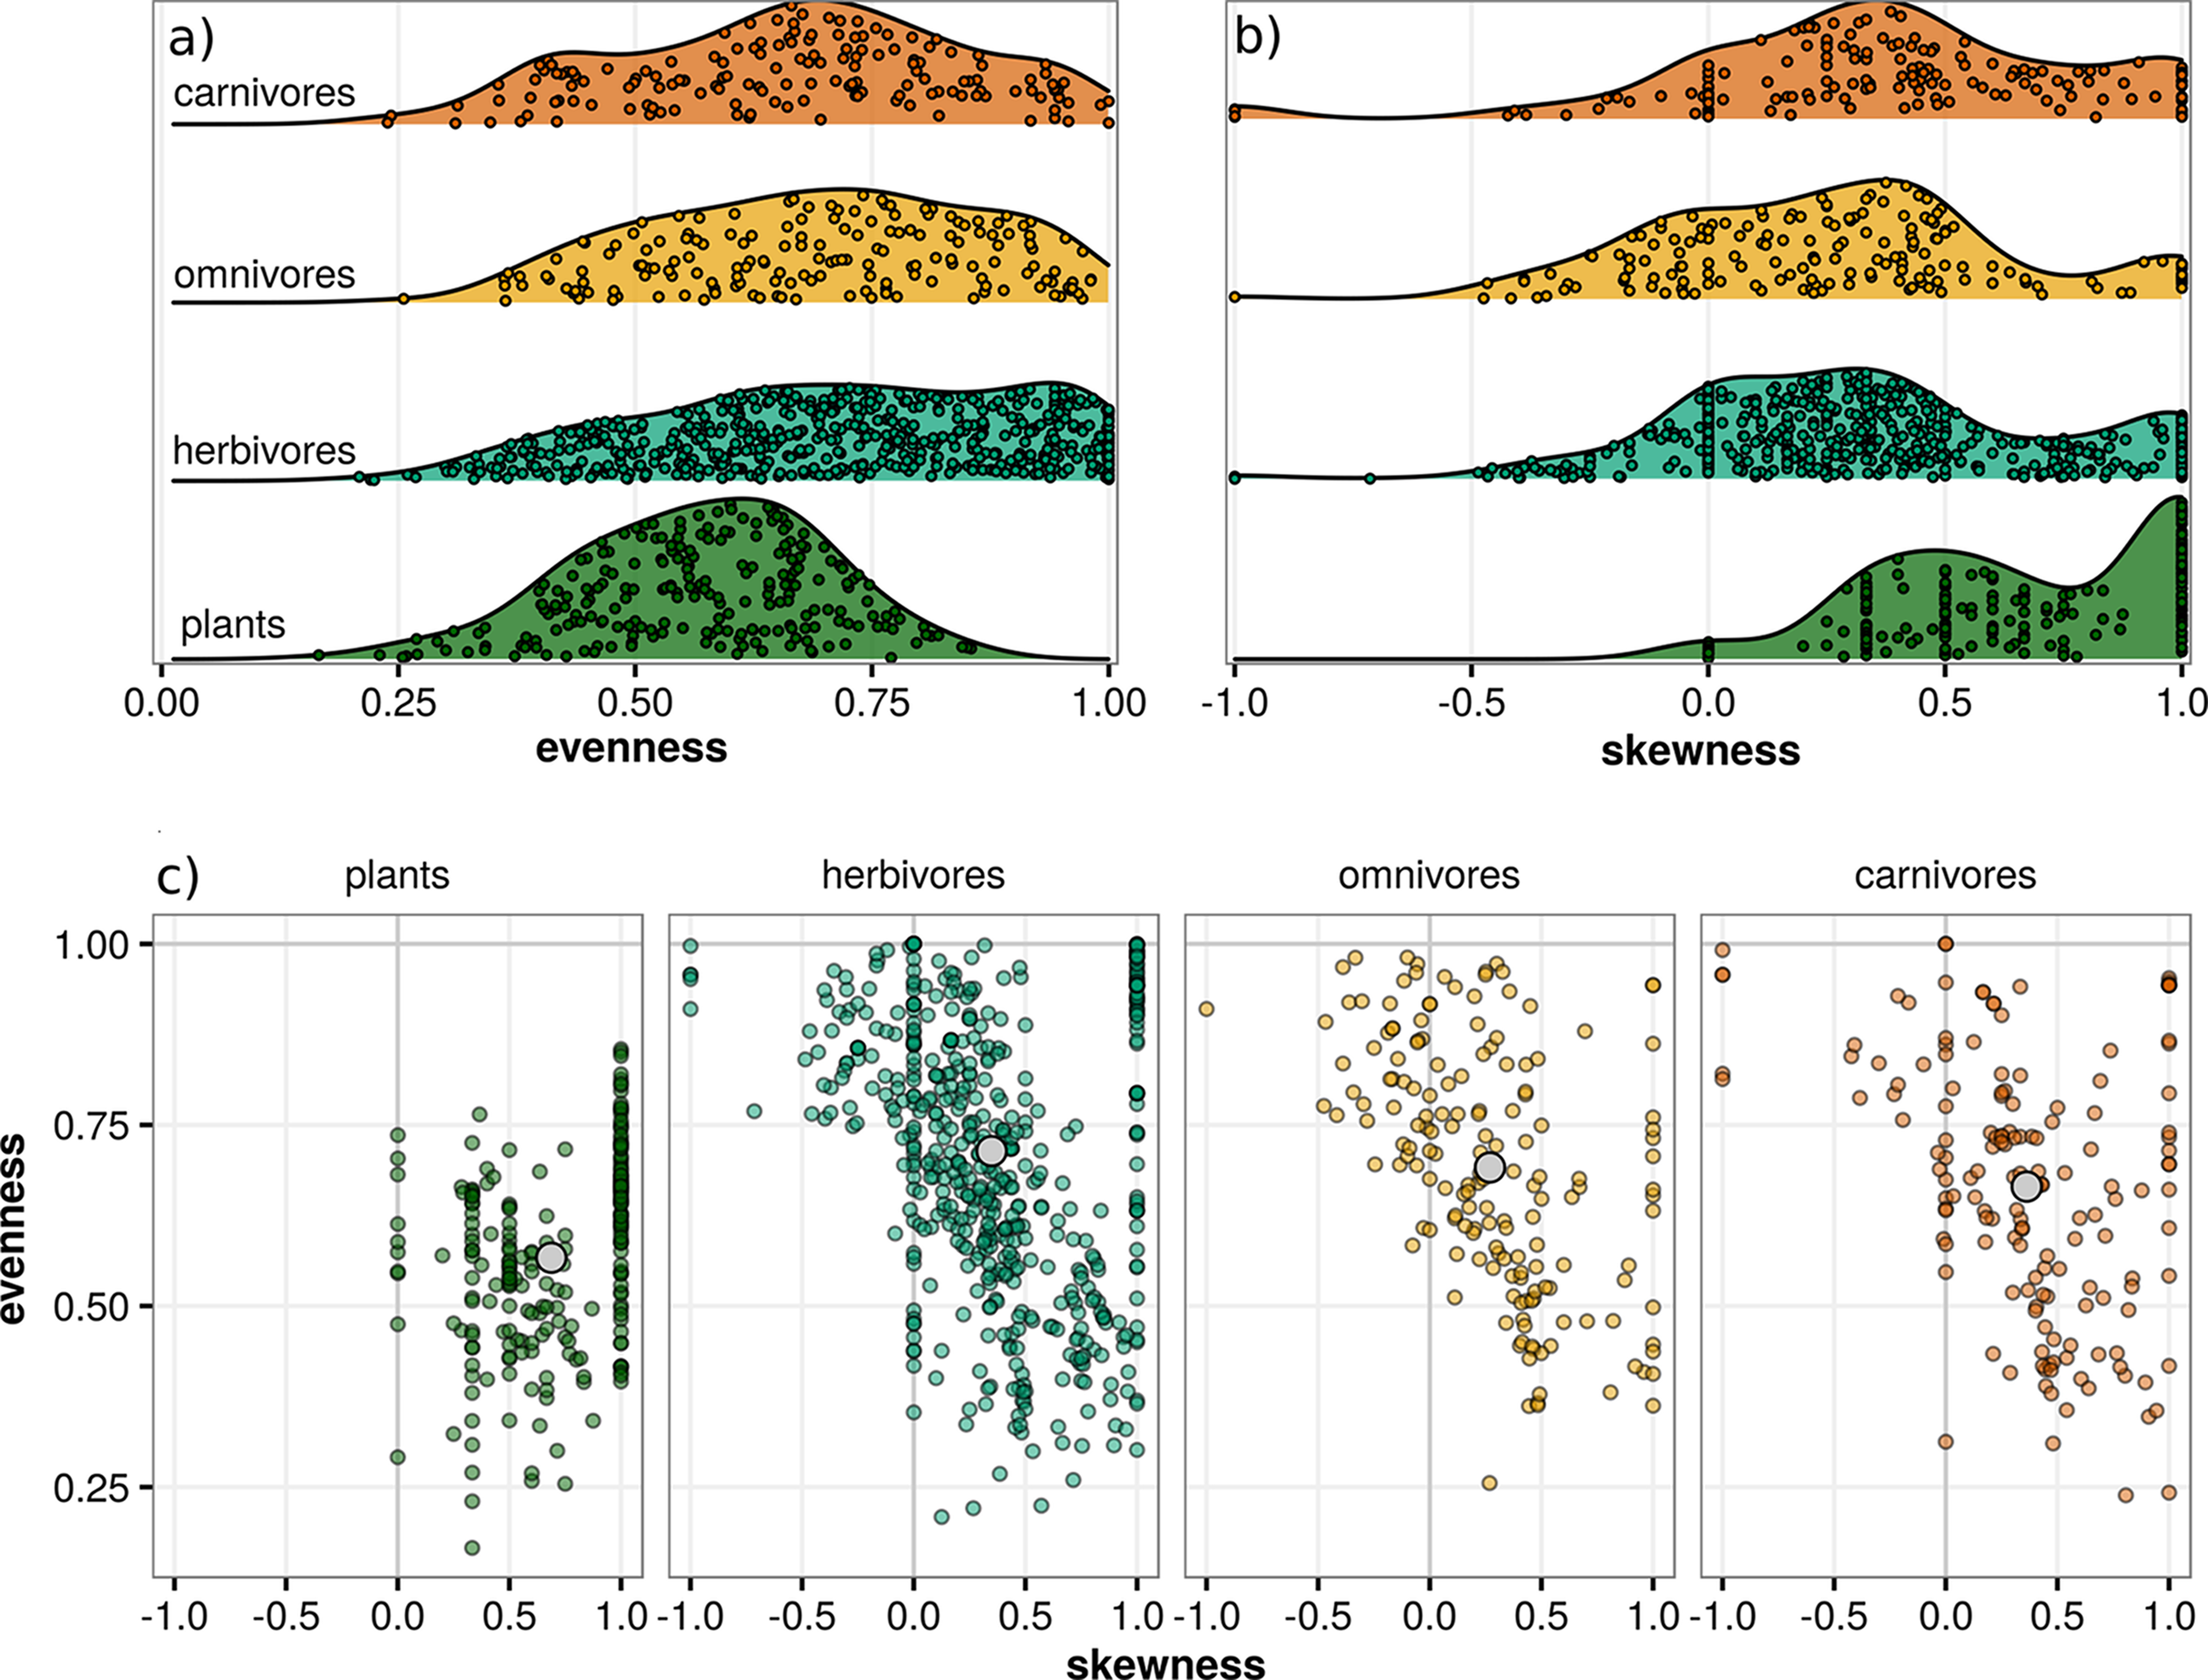
\includegraphics[width=\textwidth,height=\textheight,keepaspectratio]{./Figures/chapter04/Fig_4.png}
\caption[Evenness and skewness in empirical guilds]{\color{Gray}Density distributions of evenness (a) and skewness (b) values of the guilds studied, and the combined distribution of both metrics (panel c, cf. the theoretical results of Fig \ref{fig:fig4.3}).}\label{fig:fig4.4}
\end{figure}

\begin{table}[htbp!]
\centering
\caption[Evenness model coefficients]{\color{Gray} statistical model coefficients for the evenness of the empirical datasets. See the main text for explanation of the $\mu$ and $\sigma$ parameters. The $r^2$ of the overall model is 0.39}\label{tab:tab4.3}
\begin{tabular}{lllll}
\hline
Variable & Estimate & Std. Error & t value & p-value \\
\hline
\textbf{$\mu$ link function:  cloglog} & & & &  \\
(Intercept)              & -0.509 & 0.039 & -12.824 & $<0.05$ \\
trophic.guild-herbivores   &  0.8681 & 0.055 & 15.882 & $<0.05$ \\
trophic.guild-omnivores    &  0.753 & 0.062 &  11.975 & $<0.05$ \\
trophic.guild-carnivores    &  0.711 & 0.069 & 10.382 & $<0.05$ \\
spatial.extent           & $-7.8*10^{-7}$ & $3.1*10^{-7}$ & -2.481 & $<0.05$ \\
temporal.extent          & $-3.8*10^{-3}$ & $1.3*10^{-3}$ & -2.914 & $<0.05$ \\
richness                 &  $3.2*10^{-3}$ & $2.6*10^{-4}$ & 12.126 & $<0.05$ \\
\hline
\textbf{$\sigma$ link function:  logit} & & & & \\
(Intercept)              & -0.98 & 0.106 & -9.273 & $<0.05$ \\
trophic.guild-herbivores   &  0.969 & 0.117 &  8.251 & $<0.05$ \\
trophic.guild-omnivores    &  0.461 & 0.135 &  3.407 & $<0.05$ \\
trophic.guild-carnivores   &  0.819 & 0.143 &  5.709 & $<0.05$ \\
spatial.extent            &$-1.4*10^{-7}$ & $3.9*10^{-7}$ & -0.359 & 0.719 \\
temporal.extent           &$-6.1*10^{-4}$ & $1.5*10^{-3}$ & -0.401 & 0.688 \\
richness                  &$-3.1*10^{-3}$ & $8.6*10^{-4}$ & -3.624 & $<0.05$ \\
\hline
\end{tabular}

\end{table}

The final model for skewness included trophic guild and richness as the only predictors. Again, there were significant differences between plant and mammal guilds in their average skewness (Table \ref{tab:tab4.4}). Plant and mammal guilds were different mainly when considering low and positive skewness levels, where plants showed the highest average skewness, followed by a drop in all mammal guilds, which showed no statistical differences (Fig. \ref{fig:fig4.4}, Appendix A.4.1: Table A.4.1.2). Again, a similar qualitative trend is observed in the theoretical model (Fig. \ref{fig:fig4.3}). The effect of richness is positive, but only significant for the variation between low and highly positive skewness values (Table \ref{tab:tab4.4}).

\begin{table}[htbp!]
\centering
\caption[Skewness model coefficients]{\color{Gray} statistical model coefficients for the skewness of the empirical datasets. The $r^2$ of the model is 0.15}\label{tab:tab4.4}
\begin{tabular}{llllll}
\hline
Variable & category & Estimate & Std. Error & z score & p-value \\
\hline
(Intercept)              & (0.5,1] & -0.038 & 0.268 & -0.143  & 0.88 \\
                         & [-1,-0.5) & -5.773  & 0.688 & -8.39 & $<0.05$ \\
\begin{tabular}[c]{@{}l@{}}trophic.guild\\ herbivores \end{tabular} & (0.5,1] & -0.882 & 0.276 & -3.198 & $<0.05$ \\
                         & [-1,-0.5) & 3.138 & 0.478 & 6.571 & $<0.05$ \\
\begin{tabular}[c]{@{}l@{}}trophic.guild\\ omnivores \end{tabular}    & (0.5,1] & -1.492  & 0.342 & -4.362 & $<0.05$ \\
                         & [-1,-0.5) &  2.322 & 0.788 & 2.946  & $<0.05$ \\
\begin{tabular}[c]{@{}l@{}}trophic.guild\\ carnivores \end{tabular}    & (0.5,1] & -0.832 & 0.327 & -2.548 & $<0.05$ \\
                         & [-1,-0.5) & 4.354 & 0.492 & 8.854 & $<0.05$ \\
richness                 & (0.5,1] & 0.012 & 0.003 & 4.427   & $<0.05$ \\
                         & [-1,-0.5) & -0.314 & 0.224  & -1.397 & 0.16 \\
\hline
\end{tabular}

\end{table}

\FloatBarrier

The three mammal trophic guilds show similar negative correlations between dominance and richness (panel (a) of Fig. \ref{fig:fig4.5}, Pearson's $\rho$: -0.62 for herbivores, -0.66 for omnivores, -0.64 for carnivores). Regarding the relative rarity of the different guilds (panel (b) of Fig. \ref{fig:fig4.5}), herbivores have the same proportion of species than of individuals in local communities (Wilcoxon signed-rank test, $W = 131422, p = 0.14$, Appendix A.4.1: Table A.4.1.3), whereas omnivores are comparatively more common (i.e. there are higher relative numbers of omnivore individuals than species, $W = 162226, p < 0.05$) and carnivores are rarer (there are more carnivore species than individuals, $W = 18772, p < 0.05$).

\begin{figure}[ht]
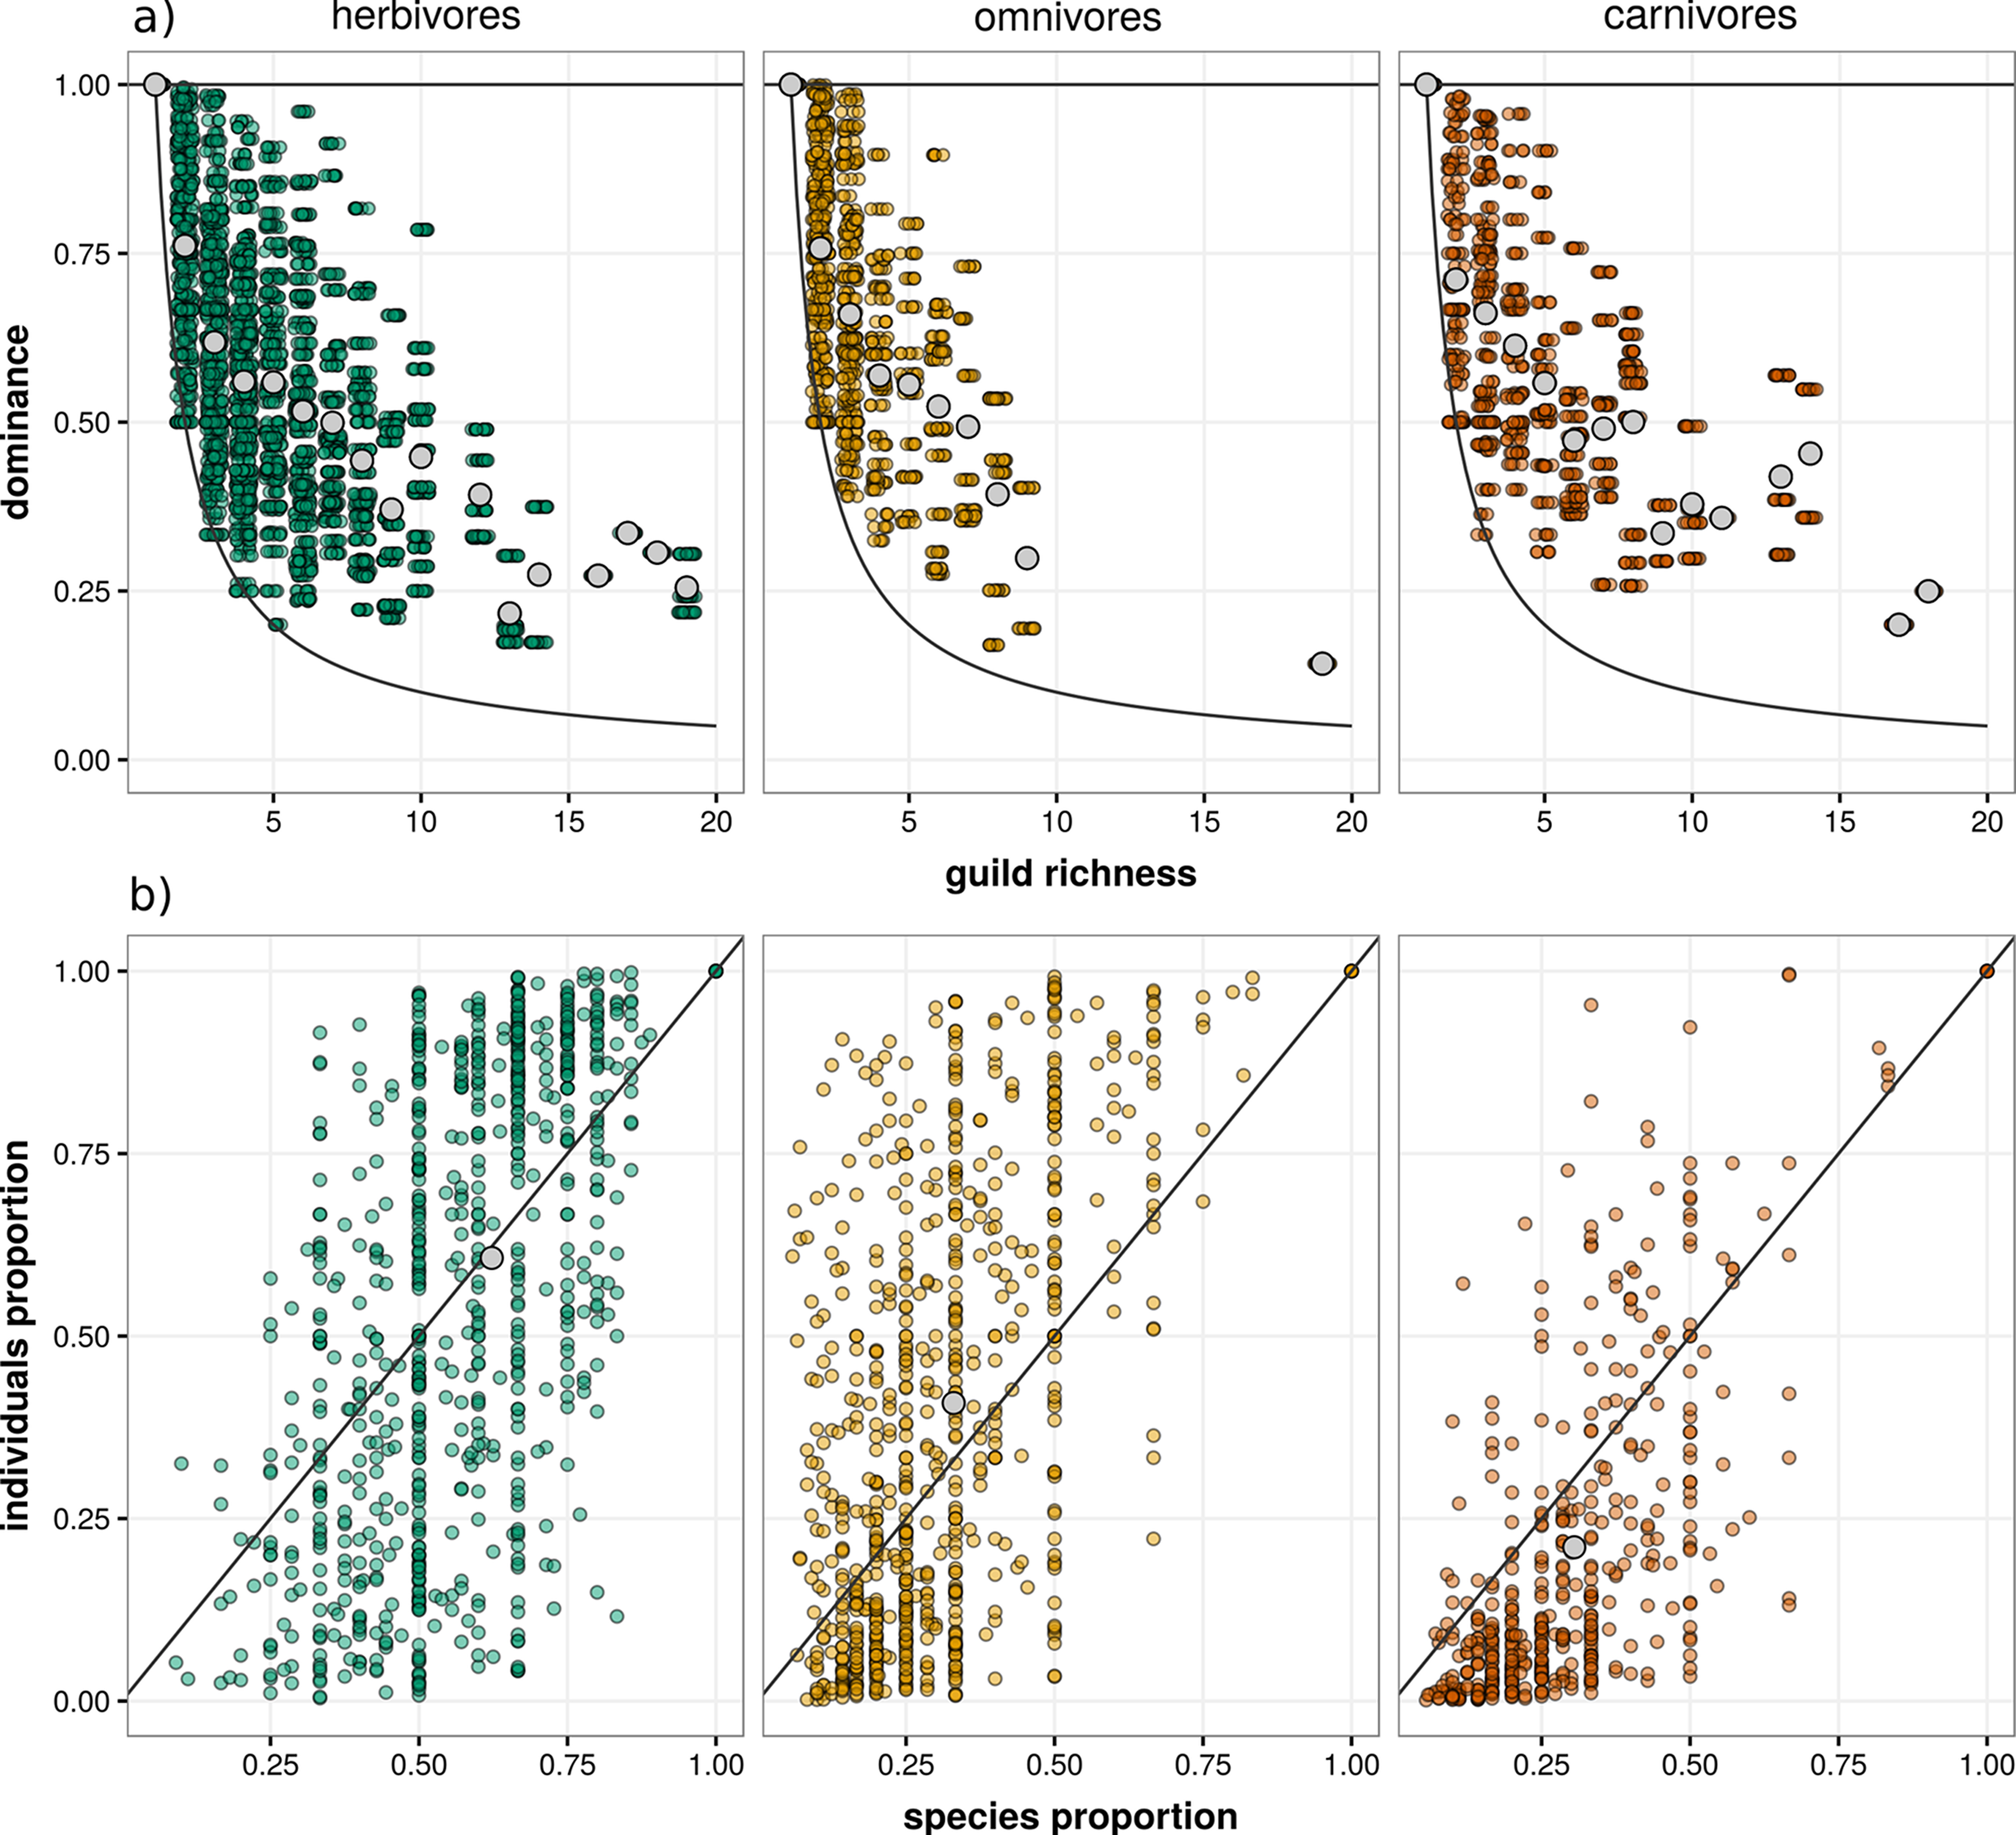
\includegraphics[width=\textwidth,height=\textheight,keepaspectratio]{./Figures/chapter04/Fig_5.png}
\caption[Species/indiv. proportion and dominance in guilds]{\color{Gray} Patterns of dominance, and the proportion of species and individuals of the mammal guilds across sampling sites, where each point is a sampling site. Dominance (upper panel) is defined as the number of individuals of the most abundant species in the guild relative to all individuals from that guild. Minimum and maximum potential dominances are represented by solid curves. The maximum level of richness shown here, for visibility, is 20 species. The lower panel shows the proportion of individuals of a given guild against the proportion of species of the same guild, and the x=y line is shown for visibility. Grey-colored dots in both panels represent average values.}\label{fig:fig4.5}
\end{figure}

\section{Discussion}

In local communities, the division of species in trophic guilds is informative with regards to the distribution of interactions and biomass flows in the community \citep{Lindeman1942, Kefi2016a}, but everything else being equal, it is unclear wheter SAD metrics are influenced by the trophic position of a guild in the local community. Here I have shown that there are significant differences between the local SADs of terrestrial plant guilds (primary producers) and different guilds of terrestrial mammals, with plant SADs being less even and more skewed than mammal ones. Furthermore, the empirical relationship between SAD metrics and trophic guild is also mediated by species richness and the spatiotemporal extent of the sample. A theoretical model combining network structure and niche apportionment schemes shows qualitatively similar trends in the variability of SAD shape across trophic guilds.

There are several potential ways of generating theoretical predictions about the variability of SAD metrics with trophic guild. Recent extensions to the theory of island biogeography \citep{Holt2009a, Gravel2011} make explicit the differences and feedbacks between species in discrete food chains, and could potentially be extended to predict the variability in species abundances across trophic levels. The model presented here, in turn, is meant to explore the role of local community structure in communities with a fixed number of species and no dynamic migration. In particular, the main question behind it is to explore whether variations in community structure (represented by species richness and network connectance) influence SAD shape of the increasing trophic guilds in model food webs.

I have shown that, given the assumptions of the model, evenness is highest (and skewness lowest) for herbivore species, and decreases for omnivore and carnivore guilds. Furthermore, community structure has significant impacts on both metrics: both richness and connectance have generally negative effects on guild evenness, and positive effects on the skewness of the SAD. With increasing richness or connectance, there is an associated increase in the number of trophic links for each species (its degree), so the general explanation for these patterns is that, under random fraction apportionment of resources, higher levels of resource overlap of the species within a given trophic guild drive higher heterogeneity in abundance distributions. Other niche apportionment schemes are likely to display different abundance patterns. For example, the \textit{dominance preemption} scheme tends to produce highly heterogeneous distribution of resources and greater dominance levels than the random fraction apportionment. On the other hand, the \textit{dominance decay} scheme will generate increasingly even abundance distributions with increasing richness or connectance \citep{Tokeshi1990}.

The empirical datasets analyzed here differ from the theoretical model in several fundamental aspects. Importantly, these datasets are likely to represent open communities, in which both core and transient species are observed, which has important implications for the associated SAD \citep{Magurran2003}. Furthermore, they are not derived from entire communities sampled across trophic guilds, but are rather a compilation in which species are classified afterwards into broad guilds (see Methods). Therefore, analogies between the theoretical results and the empirical patterns should be approached with caution, due to these important confounding factors. However, the qualitatively similar variation of SAD metrics with trophic guild observed in theoretical (Fig. \ref{fig:fig4.3}) and empirical data (Fig. \ref{fig:fig4.4}) could also be due to empirical guilds displaying, on average, mechanisms of niche apportionment similar to the ones modelled. If we assume as a working hypothesis that some degree of niche preemption by dominant species takes place \citep{Sugihara2003}, the lower evenness and higher skewness observed in terrestrial plant communities relative to mammal ones may be explained by differences in the set of resources available to the different guilds. In particular, competitive exclusion may be higher in plant communities, leading to higher dominance of a few species, due to the comparatively small set of resources for which plants compete (light, water, and essential nutrients, \citealt{Austin1990}). Mammal guilds, in turn, may potentially have a wider variety of resources available. For example, mammal herbivores, as classified in this study and according to the \textit{EltonTraits} database used to categorize trophic guilds \citep{Wilman2014}, can feed mainly on either seeds, fruits, nectar, pollen, and a large list of other plant parts. Therefore, a high degree of specialization within a guild may reduce the importance of competition and, subsequently, the relative differences in abundance between species \citep{Sugihara2003}. Such high specialization in trophic guilds is commonly observed in ecological networks \citep{Dunne2002, Gravel2011}.

Other complementary reasons for explaining the variation in SAD metrics between plants and mammals may exist. For example, differences in traits such as movement potential, which can make rare mobile mammal species harder to document, or unavoidable sampling inconsistencies between studies. It may also be the case that plant species are able to maintain lower densities for longer periods than mammal species, thus being more easily observed. Empirical estimates of minimum viable populations indicate that some plant populations may be viable with sizes of $< 1000$ individuals \citep{Nantel1996}, a number much lower than standard estimates for the viability of vertebrate species, which range in a few thousands of individuals \citep{Reed2003}. Therefore, there may simply be more rare plant species than mammals'. Niche differentiation may also be invoked to explain the relative homogeneity in SAD metrics between mammal guilds. As it is the case with herbivores, both omnivore and carnivore guilds may utilize a wide set of resources that may, generally, prevent a high degree of competitive exclusion.

Mammal guilds also show a negative correlation between dominance and guild richness, suggesting that richer guilds may be generally more even via a decrease in relative dominance, a result in accordance with previous studies \citep{Spencer2000,Dornelas2011}. This results contrast with the theoretical model, in which evenness and richness are negatively correlated (Table \ref{tab:tab4.1}). In empirical communities, the positive richness-evenness relationship may be due to the higher habitat complexity observed in richer communities \citep{Hurlbert2004}, a factor not included in the model that may lead to more diverse sets of resources and thus less importance of competitive exclusion. However, a negative relationship between richness and evenness has also been documented in different trophic guilds of grassland ecosystems \citep{Bock2007}. These contrasting results emphasize the need for controlled observations across different ecosystem types and productivity gradients. The only significant difference between mammal guilds found in this study is the relative rarity of carnivore species compared to those of other guilds, which also corroborates earlier results by \cite{Spencer2000} on invertebrate communities. Overall, these broad-scale results will undoubtedly vary across habitat types, depending on the specific sets of resources available to each guild, and on the local environmental conditions, which may have contrasting effects on the different trophic guilds \citep{Voigt2003}.

All the results presented here assume that trophic interactions are the main driver of variation in species abundances across guilds. In the theoretical results, bottom-up energy flows from trophic interactions are the only ones considered, and the mammal communities were grouped considering only a general trophic guild classification of the species. This approximation is clearly a simplification of the complex networks of interactions observed in nature, which may generate strong top-down or indirect feedbacks \citep{Menge1995, Montoya2009a}. The persistence and abundance of all species in a community is further influenced by the whole set of interactions in which they engage, among other factors \citep{Pocock2012, Garcia-Callejas2018a}. However, the distribution and frequency of most non-trophic interactions in empirical communities is not known, so no hypothesis can be formulated at this point regarding their influence on local SADs. In communities in which non-trophic interactions are known, functional guilds can be differentiated by accounting for the set of all interactions in which they engage rather than just trophic ones \citep{Sander2015,Kefi2016a}; this functional grouping may further reduce intraguild functional variability and thus increase across-guild differences, better reflecting differences in SAD shape across guilds. On the other hand, there is virtually an unlimited number of functional guilds in nature, and establishing a general, cohesive, and manageable set of functional guilds that can be applied to group every potential community seems unfeasible for the time being. Therefore, grouping by trophic guild represents a compromise between generality (as every community can be divided in such manner) and intraguild versus across-guild variability.

In any case, the variability in SAD metrics across trophic guilds of a community, and its relationship with other factors, would be better explored with dedicated sampling campaigns of different trophic guilds in multi-trophic communities, in which properties such as trophic specialization can also be tracked. This could be carried out, for example, in pond mesocosms in which most species are confined to the pond habitat, or for terrestrial habitats, in small islands where complete censuses of different trophic guilds are feasible.

The existence of an intrinsic variability in SAD shape across functional guilds has important consequences for both fundamental and applied community ecology. In theoretical models, the contributions of intraguild and interguild interactions need to be integrated in a general mechanistic framework, in order for their relative importance to be estimated. This shift from intraguild, competitive interactions to multi-trophic, community scale thinking is a necessary step forward in theoretical community ecology \citep{Chesson2008,Godoy2018,Seibold2018}. Empirical analyses of SADs would also benefit from incorporating information about the communities that harbor the guilds under study. In studies analyzing intraguild drivers of SAD shape, the community context of the study should be used to establish null expectations of interguild influence, for example, based on network structural patterns. If the guilds under study are not functionally homogeneous (e.g. taxonomic assemblages sensu \citealt{Fauth1996}) deriving mechanistic explanations about SAD shape is usually not possible, due to interspecific differences in resource use, trophic position, etc. In such descriptive studies, therefore, the community context is unnecessary. Meta-analyses of Species Abundance Distributions have shown great disparity regarding the most appropriate statistical models for fitting SADs \citep{Ulrich2010,Baldridge2016}. If the results presented here hold, accounting for this null expectation may help clarify which statistical models are best suited to fit each set of data.

\section{Conclusions}

Species Abundance Distributions have many axes of variability. Here I have showed that intrinsic differences exist between the SAD of terrestrial plant and mammal communities. Plant communities are significantly less even and more skewed than mammal ones, and there are no significant differences in either metric between the mammal trophic guilds considered. This result may arise from differences in niche availability for the different guilds, following the hypothesis that higher niche availability implies a higher evenness in species abundances. Although these results are derived from extensive datasets controlling for several factors, targeted studies are needed to further confirm this pattern and test it in a variety of systems. This prospective line of research would shed new light on both theoretical and applied analyses of Species Abundance Distributions, and would help in the integration of classic horizontal community ecology patterns in the context of communities encompassing multiple trophic levels and interaction types.

%-----------------------------------------------------------------
